\documentclass[11pt,fleqn, openany]{book} % Default font size and left-justified equations

%%%%%%%%%%%%%%%%%%%%%%%%%%%%%%%%%%%%%%%%%
% The Legrand Orange Book
% Structural Definitions File
% Version 2.1 (26/09/2018)
%
% Original author:
% Mathias Legrand (legrand.mathias@gmail.com) with modifications by:
% Vel (vel@latextemplates.com)
% 
% This file was downloaded from:
% http://www.LaTeXTemplates.com
%
% License:
% CC BY-NC-SA 3.0 (http://creativecommons.org/licenses/by-nc-sa/3.0/)
%
%%%%%%%%%%%%%%%%%%%%%%%%%%%%%%%%%%%%%%%%%

%----------------------------------------------------------------------------------------
%	VARIOUS REQUIRED PACKAGES AND CONFIGURATIONS
%----------------------------------------------------------------------------------------

\usepackage[table]{xcolor}

\usepackage{graphicx}
\usepackage{tabularx} % Required for including pictures
\usepackage{pgf,tikz,tkz-tab,eurosym,yhmath, stmaryrd}
\usepackage{pgfplots}
\usepackage{mathrsfs}
\usetikzlibrary{patterns}
\usetikzlibrary{trees}
\graphicspath{{../../Pictures/}}
\usepackage{multicol} 


\usepackage[english]{babel} % English language/hyphenation
\usepackage{icomma}
\usepackage{enumitem} % Customize lists
\setlist{nolistsep, nosep, nolistsep} % Reduce spacing between bullet points and numbered lists

\usepackage{booktabs} % Required for nicer horizontal rules in tables

 % Required for specifying colors by name


\definecolor{ocre}{RGB}{243,102,25} % Define the orange color used for highlighting throughout the book

\usepackage{listings}

\definecolor{codegreen}{rgb}{0,0.6,0}
\definecolor{codegray}{rgb}{0.5,0.5,0.5}
\definecolor{codepurple}{rgb}{0.58,0,0.82}
\definecolor{backcolour}{rgb}{0.95,0.95,0.92}

\lstdefinestyle{mystyle}{
    backgroundcolor=\color{backcolour},   
    commentstyle=\color{codegreen},
    keywordstyle=\color{magenta},
    numberstyle=\tiny\color{codegray},
    stringstyle=\color{codepurple},
    basicstyle=\ttfamily\footnotesize,
    breakatwhitespace=false,         
    breaklines=true,                 
    captionpos=b,                    
    keepspaces=true,                 
    numbers=left,                    
    numbersep=5pt,                  
    showspaces=false,                
    showstringspaces=false,
    showtabs=false,                  
    tabsize=2
}

\lstset{style=mystyle}

%----------------------------------------------------------------------------------------
% Paramétrage XSIM
%----------------------------------------------------------------------------------------

\usepackage[no-files]{xsim}


\DeclareExerciseEnvironmentTemplate{myex}{%
    \textbf{%
      \hypertarget{ex:\ExerciseID}{\sffamily{\ensuremath{\blacktriangleright}} Exercice \GetExerciseProperty{counter} \GetExerciseProperty{subtitle} --}
      \hyperlink{sol:\ExerciseID}{Voir le corrigé}%
    }\par
}{\par\smallskip}

\DeclareExerciseEnvironmentTemplate{mysol}{%
    \textbf{%
      \hypertarget{sol:\ExerciseID}{\sffamily{\ensuremath{\blacktriangleright}} Correction \GetExerciseProperty{counter} --}
      \hyperlink{ex:\ExerciseID}{Voir l'énoncé}%
    }\par
}{\par\medskip}

\xsimsetup{
  exercise/template = myex ,
  solution/template = mysol 
}

%Collection exercices

\DeclareExerciseTagging{topic}

\xsimsetup{collect}

%----------------------------------------------------------------------------------------
% SYMBOLES
%----------------------------------------------------------------------------------------

\newcommand\imCMsym[4][\mathord]{%
  \DeclareFontFamily{U} {#2}{}
  \DeclareFontShape{U}{#2}{m}{n}{
    <-6> #25
    <6-7> #26
    <7-8> #27
    <8-9> #28
    <9-10> #29
    <10-12> #210
    <12-> #212}{}
  \DeclareSymbolFont{CM#2} {U} {#2}{m}{n}
  \DeclareMathSymbol{#4}{#1}{CM#2}{#3}
}
\newcommand\alsoimCMsym[4][\mathord]{\DeclareMathSymbol{#4}{#1}{CM#2}{#3}}

\imCMsym{cmmi}{124}{\CMjmath}

\newcommand{\Oij}{(O\,;\,\vec{\imath}\,,\, \vec{\CMjmath} )}
\newcommand{\Oijk}{(O\,;\,\vec{\imath}\,,\, \vec{\CMjmath}\,,\,\vec{k})}

\newcommand\e{\mathrm{e}}
\newcommand\R{\mathbb{R}}
\newcommand\N{\mathbb{N}}


%----------------------------------------------------------------------------------------
%	MARGINS
%----------------------------------------------------------------------------------------

\usepackage{geometry} % Required for adjusting page dimensions and margins

\geometry{
	paper=a4paper, % Paper size, change to letterpaper for US letter size
	top=3cm, % Top margin
	bottom=3cm, % Bottom margin
	left=2cm, % Left margin
	right=2cm, % Right margin
	headheight=14pt, % Header height
	footskip=1.4cm, % Space from the bottom margin to the baseline of the footer
	headsep=10pt, % Space from the top margin to the baseline of the header
	%showframe, % Uncomment to show how the type block is set on the page
}

\setlength{\parindent}{0pt}
\parskip=5pt



%----------------------------------------------------------------------------------------
%	FONTS
%----------------------------------------------------------------------------------------

\usepackage{avant} % Use the Avantgarde font for headings
\usepackage{times} % Use the Times font for headings
\usepackage{mathptmx} % Use the Adobe Times Roman as the default text font together with math symbols from the Sym­bol, Chancery and Com­puter Modern fonts

%\usepackage{microtype} % Slightly tweak font spacing for aesthetics
%\usepackage[utf8]{inputenc} % Required for including letters with accents
\usepackage[T1]{fontenc} % Use 8-bit encoding that has 256 glyphs

%----------------------------------------------------------------------------------------
%	BIBLIOGRAPHY AND INDEX
%----------------------------------------------------------------------------------------

\usepackage[style=numeric,citestyle=numeric,sorting=nyt,sortcites=true,autopunct=true,babel=hyphen,hyperref=true,abbreviate=false,backref=true,backend=biber]{biblatex}
\addbibresource{bibliography.bib} % BibTeX bibliography file
\defbibheading{bibempty}{}

\usepackage{calc} % For simpler calculation - used for spacing the index letter headings correctly
\usepackage{makeidx} % Required to make an index
\makeindex % Tells LaTeX to create the files required for indexing

%----------------------------------------------------------------------------------------
%	MAIN TABLE OF CONTENTS
%----------------------------------------------------------------------------------------

\usepackage{titletoc} % Required for manipulating the table of contents

\contentsmargin{0cm} % Removes the default margin

% Part text styling (this is mostly taken care of in the PART HEADINGS section of this file)
\titlecontents{part}
	[0cm] % Left indentation
	{\addvspace{20pt}\bfseries} % Spacing and font options for parts
	{}
	{}
	{}

% Chapter text styling
\titlecontents{chapter}
	[1.25cm] % Left indentation
	{\addvspace{12pt}\large\sffamily\bfseries} % Spacing and font options for chapters
	{\color{ocre!60}\contentslabel[\Large\thecontentslabel]{1.25cm}\color{ocre}} % Formatting of numbered sections of this type
	{\color{ocre}} % Formatting of numberless sections of this type
	{\color{ocre!60}\normalsize\;\titlerule*[.5pc]{.}\;\thecontentspage} % Formatting of the filler to the right of the heading and the page number

% Section text styling
\titlecontents{section}
	[1.25cm] % Left indentation
	{\addvspace{3pt}\sffamily\bfseries} % Spacing and font options for sections
	{\contentslabel[\thecontentslabel]{1.25cm}} % Formatting of numbered sections of this type
	{} % Formatting of numberless sections of this type
	{\hfill\color{black}\thecontentspage} % Formatting of the filler to the right of the heading and the page number

% Subsection text styling
\titlecontents{subsection}
	[1.25cm] % Left indentation
	{\addvspace{1pt}\sffamily\small} % Spacing and font options for subsections
	{\contentslabel[\thecontentslabel]{1.25cm}} % Formatting of numbered sections of this type
	{} % Formatting of numberless sections of this type
	{\ \titlerule*[.5pc]{.}\;\thecontentspage} % Formatting of the filler to the right of the heading and the page number

% Figure text styling
\titlecontents{figure}
	[1.25cm] % Left indentation
	{\addvspace{1pt}\sffamily\small} % Spacing and font options for figures
	{\thecontentslabel\hspace*{1em}} % Formatting of numbered sections of this type
	{} % Formatting of numberless sections of this type
	{\ \titlerule*[.5pc]{.}\;\thecontentspage} % Formatting of the filler to the right of the heading and the page number

% Table text styling
\titlecontents{table}
	[1.25cm] % Left indentation
	{\addvspace{1pt}\sffamily\small} % Spacing and font options for tables
	{\thecontentslabel\hspace*{1em}} % Formatting of numbered sections of this type
	{} % Formatting of numberless sections of this type
	{\ \titlerule*[.5pc]{.}\;\thecontentspage} % Formatting of the filler to the right of the heading and the page number

%----------------------------------------------------------------------------------------
%	MINI TABLE OF CONTENTS IN PART HEADS
%----------------------------------------------------------------------------------------

% Chapter text styling
\titlecontents{lchapter}
	[0em] % Left indentation
	{\addvspace{15pt}\large\sffamily\bfseries} % Spacing and font options for chapters
	{\color{ocre}\contentslabel[\Large\thecontentslabel]{1.25cm}\color{ocre}} % Chapter number
	{}  
	{\color{ocre}\normalsize\sffamily\bfseries\;\titlerule*[.5pc]{.}\;\thecontentspage} % Page number

% Section text styling
\titlecontents{lsection}
	[0em] % Left indentation
	{\sffamily\small} % Spacing and font options for sections
	{\contentslabel[\thecontentslabel]{1.25cm}} % Section number
	{}
	{}

% Subsection text styling (note these aren't shown by default, display them by searchings this file for tocdepth and reading the commented text)
\titlecontents{lsubsection}
	[.5em] % Left indentation
	{\sffamily\footnotesize} % Spacing and font options for subsections
	{\contentslabel[\thecontentslabel]{1.25cm}}
	{}
	{}

%----------------------------------------------------------------------------------------
%	HEADERS AND FOOTERS
%----------------------------------------------------------------------------------------


\usepackage{fancyhdr} % Required for header and footer configuration

\pagestyle{fancy}
\renewcommand{\chaptermark}[1]{\markboth{\sffamily\normalsize\bfseries\ \thechapter.\ #1}{}} % Chapter text font settings
\renewcommand{\sectionmark}[1]{\markright{\sffamily\normalsize\thesection\hspace{5pt}#1}{}} % Section text font settings
\fancyhf{} \fancyhead[LE,RO]{\sffamily\normalsize\thepage} % Font setting for the page number in the header
\fancyhead[LO]{\rightmark} % Print the nearest section name on the left side of odd pages
\fancyhead[RE]{\leftmark} % Print the current chapter name on the right side of even pages

\fancyfoot[L]{Jason LAPEYRONNIE}
\fancyfoot[R]{\href{http://mathoutils.fr}{http://mathoutils.fr}} % Uncomment to include a footer

\renewcommand{\headrulewidth}{0.5pt} % Thickness of the rule under the header
\renewcommand{\footrulewidth}{0.5pt} % Thickness of the rule under the header

\fancypagestyle{plain}{% Style for when a plain pagestyle is specified
	\fancyhead{}\renewcommand{\headrulewidth}{0pt}%
}

% Removes the header from odd empty pages at the end of chapters
\makeatletter
\renewcommand{\cleardoublepage}{
\clearpage\ifodd\c@page\else
\hbox{}
\vspace*{\fill}
\thispagestyle{empty}
\newpage
\fi}

%----------------------------------------------------------------------------------------
%	THEOREM STYLES
%----------------------------------------------------------------------------------------

\usepackage{amsmath,amsfonts,amssymb,amsthm} % For math equations, theorems, symbols, etc

\newcommand{\intoo}[2]{\mathopen{]}#1\,;#2\mathclose{[}}
\newcommand{\ud}{\mathop{\mathrm{{}d}}\mathopen{}}
\newcommand{\intff}[2]{\mathopen{[}#1\,;#2\mathclose{]}}
\renewcommand{\qedsymbol}{$\blacksquare$}
\newtheorem{notation}{Notation}[section]

% Boxed/framed environments
\newtheoremstyle{ocrenumbox}% Theorem style name
{0pt}% Space above
{0pt}% Space below
{\normalfont}% Body font
{}% Indent amount
{\small\bf\sffamily\color{ocre}}% Theorem head font
{\;:\;}% Punctuation after theorem head
{0.25em}% Space after theorem head
{\small\sffamily\color{ocre}\thmname{#1}\nobreakspace\thmnumber{\@ifnotempty{#1}{}\@upn{#2}}% Theorem text (e.g. Theorem 2.1)
\thmnote{\nobreakspace\the\thm@notefont\sffamily\bfseries\color{black}---\nobreakspace#3}} % Optional theorem note

\newtheoremstyle{blacknumex}% Theorem style name
{5pt}% Space above
{10pt}% Space below
{\normalfont}% Body font
{} % Indent amount
{\small\bf\sffamily}% Theorem head font
{\;:\;}% Punctuation after theorem head
{0.25em}% Space after theorem head
{\small\sffamily{\tiny\ensuremath{\blacksquare}}\nobreakspace\thmname{#1}\nobreakspace\thmnumber{\@ifnotempty{#1}{}\@upn{#2}}% Theorem text (e.g. Theorem 2.1)
\thmnote{\nobreakspace\the\thm@notefont\sffamily\bfseries---\nobreakspace#3}}% Optional theorem note

\newtheoremstyle{blacknumexo}% Theorem style name
{15pt}% Space above
{10pt}% Space below
{\normalfont}% Body font
{} % Indent amount
{\small\bf\sffamily}% Theorem head font
{}% Punctuation after theorem head
{0.5em}% Space after theorem head
{\small\sffamily{\ensuremath{\blacktriangleright}}\nobreakspace\thmname{#1}\nobreakspace\thmnumber{\@ifnotempty{#1}{}\@upn{#2}}% Theorem text (e.g. Theorem 2.1)
\thmnote{\nobreakspace\the\thm@notefont\sffamily\bfseries---\nobreakspace#3} \\}% Optional theorem note



\newtheoremstyle{blacknumbox} % Theorem style name
{0pt}% Space above
{5pt}% Space below
{}% Body font
{}% Indent amount
{\large\bf\sffamily}% Theorem head font
{\;:\;}% Punctuation after theorem head
{0.25em}% Space after theorem head
{\small\sffamily\thmname{#1}\nobreakspace\thmnumber{\@ifnotempty{#1}{}\@upn{#2}}% Theorem text (e.g. Theorem 2.1)
\thmnote{\nobreakspace\the\thm@notefont\sffamily\bfseries---\nobreakspace#3}}% Optional theorem note

% Non-boxed/non-framed environments
\newtheoremstyle{ocrenum}% Theorem style name
{5pt}% Space above
{5pt}% Space below
{\normalfont}% Body font
{}% Indent amount
{\small\bf\sffamily\color{ocre}}% Theorem head font
{\;:\;}% Punctuation after theorem head
{0.25em}% Space after theorem head
{\small\sffamily\color{ocre}\thmname{#1}\nobreakspace\thmnumber{\@ifnotempty{#1}{}\@upn{#2}}% Theorem text (e.g. Theorem 2.1)
\thmnote{\nobreakspace\the\thm@notefont\sffamily\bfseries\color{black}---\nobreakspace#3}} % Optional theorem note
\makeatother

% Defines the theorem text style for each type of theorem to one of the three styles above
\newcounter{dummy} 
\newcounter{thm}
\newcounter{correction}
\newcounter{qst}
\theoremstyle{ocrenumbox}
\newtheorem{theoremeT}[dummy]{Théorème}
\newtheorem{exerciseT}{Propriété}
\newtheorem{principeT}{Principe}
\theoremstyle{blacknumex}
\newtheorem{exampleT}{Exemple}
\theoremstyle{blacknumexo}
\newtheorem{exo}[thm]{Exercice}
\newtheorem{corr}[correction]{Correction}
\newtheorem{quest}[qst]{Question}
\theoremstyle{blacknumbox}
\newtheorem{vocabulary}{Vocabulary}[section]
\newtheorem{definitionT}{Définition}
\newtheorem{corollaryT}[dummy]{Corollary}
\theoremstyle{ocrenum}
\newtheorem{proofT}[dummy]{Démonstration}


%----------------------------------------------------------------------------------------
%	DEFINITION OF COLORED BOXES
%----------------------------------------------------------------------------------------

\RequirePackage[framemethod=default]{mdframed} % Required for creating the theorem, definition, exercise and corollary boxes

% Theorem box
\newmdenv[skipabove=7pt,
skipbelow=7pt,
backgroundcolor=black!5,
linecolor=ocre,
innerleftmargin=5pt,
innerrightmargin=5pt,
innertopmargin=10pt,
leftmargin=0cm,
rightmargin=0cm,
innerbottommargin=5pt]{tBox}

%Proposition box	  
\newmdenv[skipabove=7pt,
skipbelow=7pt,
rightline=false,
leftline=true,
topline=false,
bottomline=false,
backgroundcolor=ocre!10,
linecolor=ocre,
innerleftmargin=5pt,
innerrightmargin=5pt,
innertopmargin=10pt,
innerbottommargin=3pt,
leftmargin=0cm,
rightmargin=0cm,
linewidth=4pt]{eBox}	

% Definition box
\newmdenv[skipabove=7pt,
backgroundcolor=ocre!4,
skipbelow=7pt,
rightline=false,
leftline=true,
topline=false,
bottomline=false,
linecolor=ocre,
innerleftmargin=5pt,
innerrightmargin=5pt,
innertopmargin=10pt,
leftmargin=0cm,
rightmargin=0cm,
linewidth=4pt,
innerbottommargin=5pt]{dBox}	

% Corollary box
\newmdenv[skipabove=7pt,
skipbelow=7pt,
rightline=false,
leftline=true,
topline=false,
bottomline=false,
linecolor=gray,
backgroundcolor=black!5,
innerleftmargin=5pt,
innerrightmargin=5pt,
innertopmargin=5pt,
leftmargin=0cm,
rightmargin=0cm,
linewidth=4pt,
innerbottommargin=5pt]{cBox}

\newmdenv[skipabove=7pt,
skipbelow=7pt,
backgroundcolor=black!5,
innerleftmargin=5pt,
topline=false,
bottomline=false,
rightline=false,
leftline=false,
innerrightmargin=5pt,
innertopmargin=5pt,
leftmargin=0cm,
rightmargin=0cm,
innerbottommargin=5pt]{xBox}

% Creates an environment for each type of theorem and assigns it a theorem text style from the "Theorem Styles" section above and a colored box from above
\newenvironment{theorem}{\begin{tBox}\begin{theoremeT}}{\end{theoremeT}\end{tBox}}

\newenvironment{exo2}{\noindent \begin{exo}\item\relax \noindent \begin{eBox}\item\relax}{\end{eBox}\end{exo}}


\newenvironment{proposition}{\begin{eBox}\begin{exerciseT}}{\hfill{\color{ocre}}\end{exerciseT}\end{eBox}}		

\newenvironment{principe}{\begin{eBox}\begin{principeT}}{\hfill{\color{ocre}}\end{principeT}\end{eBox}}	
		  
\newenvironment{definition}{\begin{dBox}\begin{definitionT}}{\end{definitionT}\end{dBox}}	

\newenvironment{example}{\begin{xBox}\begin{exampleT}}{\hfill{\tiny\ensuremath{\blacksquare}}\end{exampleT}\end{xBox}}

\newenvironment{demonstration}{\begin{proofT}}{\hfill{\tiny\ensuremath{\square}}\end{proofT}}		
\newenvironment{corollary}{\begin{cBox}\begin{corollaryT}}{\end{corollaryT}\end{cBox}}	

%----------------------------------------------------------------------------------------
%	REMARK ENVIRONMENT
%----------------------------------------------------------------------------------------

\newenvironment{remark}{\par\vspace{5pt}\small % Vertical white space above the remark and smaller font size
\begin{list}{}{
\leftmargin=25pt % Indentation on the left
\rightmargin=15pt}\item\ignorespaces % Indentation on the right
\makebox[-2.5pt]{
\begin{tikzpicture}[overlay]
\node[draw=ocre!60,line width=1pt,circle,fill=ocre!25,font=\sffamily\bfseries,inner sep=2pt,outer sep=0pt] at (-15pt,0pt){\textcolor{ocre}{R}};\end{tikzpicture}} % Orange R in a circle
\advance\baselineskip -1pt}{\end{list}\vskip5pt} % Tighter line spacing and white space after remark

%----------------------------------------------------------------------------------------
%	SECTION NUMBERING IN THE MARGIN
%----------------------------------------------------------------------------------------

\makeatletter
\renewcommand{\@seccntformat}[1]{\llap{\textcolor{ocre}{\csname the#1\endcsname}\hspace{1em}}}                    
\renewcommand{\section}{\@startsection{section}{1}{\z@}
{-4ex \@plus -1ex \@minus -.4ex}
{1ex \@plus.2ex }
{\normalfont\LARGE\sffamily\bfseries}}
\renewcommand{\subsection}{\@startsection {subsection}{2}{\z@}
{-3ex \@plus -0.1ex \@minus -.4ex}
{0.5ex \@plus.2ex }
{\normalfont\sffamily\bfseries}}
\renewcommand{\subsubsection}{\@startsection {subsubsection}{3}{\z@}
{-2ex \@plus -0.1ex \@minus -.2ex}
{.2ex \@plus.2ex }
{\normalfont\small\sffamily\bfseries}}                        
\renewcommand\paragraph{\@startsection{paragraph}{4}{\z@}
{-2ex \@plus-.2ex \@minus .2ex}
{.1ex}
{\normalfont\small\sffamily\bfseries}}

%----------------------------------------------------------------------------------------
%	PART HEADINGS
%----------------------------------------------------------------------------------------

% Numbered part in the table of contents
\newcommand{\@mypartnumtocformat}[2]{%
	\setlength\fboxsep{0pt}%
	\noindent\colorbox{ocre!20}{\strut\parbox[c][.7cm]{\ecart}{\color{ocre!70}\Large\sffamily\bfseries\centering#1}}\hskip\esp\colorbox{ocre!40}{\strut\parbox[c][.7cm]{\linewidth-\ecart-\esp}{\Large\sffamily\centering#2}}%
}

% Unnumbered part in the table of contents
\newcommand{\@myparttocformat}[1]{%
	\setlength\fboxsep{0pt}%
	\noindent\colorbox{ocre!40}{\strut\parbox[c][.7cm]{\linewidth}{\Large\sffamily\centering#1}}%
}

\newlength\esp
\setlength\esp{4pt}
\newlength\ecart
\setlength\ecart{1.2cm-\esp}
\newcommand{\thepartimage}{}%
\newcommand{\partimage}[1]{\renewcommand{\thepartimage}{#1}}%
\def\@part[#1]#2{%
\ifnum \c@secnumdepth >-2\relax%
\refstepcounter{part}%
\addcontentsline{toc}{part}{\texorpdfstring{\protect\@mypartnumtocformat{\thepart}{#1}}{\partname~\thepart\ ---\ #1}}
\else%
\addcontentsline{toc}{part}{\texorpdfstring{\protect\@myparttocformat{#1}}{#1}}%
\fi%
\startcontents%
\markboth{}{}%
{\thispagestyle{empty}%
\begin{tikzpicture}[remember picture,overlay]%
\node at (current page.north west){\begin{tikzpicture}[remember picture,overlay]%	
\fill[ocre!20](0cm,0cm) rectangle (\paperwidth,-\paperheight);
\node[anchor=north] at (4cm,-3.25cm){\color{ocre!40}\fontsize{220}{100}\sffamily\bfseries\thepart}; 
\node[anchor=south east] at (\paperwidth-1cm,-\paperheight+1cm){\parbox[t][][t]{8.5cm}{
\printcontents{l}{0}{\setcounter{tocdepth}{1}}% The depth to which the Part mini table of contents displays headings; 0 for chapters only, 1 for chapters and sections and 2 for chapters, sections and subsections
}};
\node[anchor=north east] at (\paperwidth-1.5cm,-3.25cm){\parbox[t][][t]{15cm}{\strut\raggedleft\color{white}\fontsize{30}{30}\sffamily\bfseries#2}};
\end{tikzpicture}};
\end{tikzpicture}}%
\@endpart}
\def\@spart#1{%
\startcontents%
\phantomsection
{\thispagestyle{empty}%
\begin{tikzpicture}[remember picture,overlay]%
\node at (current page.north west){\begin{tikzpicture}[remember picture,overlay]%	
\fill[ocre!20](0cm,0cm) rectangle (\paperwidth,-\paperheight);
\node[anchor=north east] at (\paperwidth-1.5cm,-3.25cm){\parbox[t][][t]{15cm}{\strut\raggedleft\color{white}\fontsize{30}{30}\sffamily\bfseries#1}};
\end{tikzpicture}};
\end{tikzpicture}}
\addcontentsline{toc}{part}{\texorpdfstring{%
\setlength\fboxsep{0pt}%
\noindent\protect\colorbox{ocre!40}{\strut\protect\parbox[c][.7cm]{\linewidth}{\Large\sffamily\protect\centering #1\quad\mbox{}}}}{#1}}%
\@endpart}
\def\@endpart{\vfil\newpage
\if@twoside
\if@openright
\null
\thispagestyle{empty}%
\newpage
\fi
\fi
\if@tempswa
\twocolumn
\fi}

%----------------------------------------------------------------------------------------
%	CHAPTER HEADINGS
%----------------------------------------------------------------------------------------

% A switch to conditionally include a picture, implemented by Christian Hupfer
\newif\ifusechapterimage
\usechapterimagetrue
\newcommand{\thechapterimage}{}%
\newcommand{\chapterimage}[1]{\ifusechapterimage\renewcommand{\thechapterimage}{#1}\fi}%
\newcommand{\autodot}{.}
\def\@makechapterhead#1{%
{\parindent \z@ \raggedright \normalfont
\ifnum \c@secnumdepth >\m@ne
\if@mainmatter
\begin{tikzpicture}[remember picture,overlay]
\node at (current page.north west)
{\begin{tikzpicture}[remember picture,overlay]
\node[anchor=north west,inner sep=0pt] at (0,0) {\ifusechapterimage\includegraphics[width=\paperwidth]{\thechapterimage}\fi};
\draw[anchor=west] (\Gm@lmargin,-3cm) node [line width=2pt,rounded corners=15pt,draw=ocre,fill=white,fill opacity=0.5,inner sep=15pt]{\strut\makebox[22cm]{}};
\draw[anchor=west] (\Gm@lmargin+.3cm,-3cm) node {\huge\sffamily\bfseries\color{black}\thechapter\autodot~#1\strut};
\end{tikzpicture}};
\end{tikzpicture}
\else
\begin{tikzpicture}[remember picture,overlay]
\node at (current page.north west)
{\begin{tikzpicture}[remember picture,overlay]
\node[anchor=north west,inner sep=0pt] at (0,0) {\ifusechapterimage\includegraphics[width=\paperwidth]{\thechapterimage}\fi};
\draw[anchor=west] (\Gm@lmargin,-3cm) node [line width=2pt,rounded corners=15pt,draw=ocre,fill=white,fill opacity=0.5,inner sep=15pt]{\strut\makebox[22cm]{}};
\draw[anchor=west] (\Gm@lmargin+.3cm,-3cm) node {\huge\sffamily\bfseries\color{black}#1\strut};
\end{tikzpicture}};
\end{tikzpicture}
\fi\fi\par\vspace*{50\p@}}}

%-------------------------------------------

\def\@makeschapterhead#1{%
\begin{tikzpicture}[remember picture,overlay]
\node at (current page.north west)
{\begin{tikzpicture}[remember picture,overlay]
\node[anchor=north west,inner sep=0pt] at (0,0) {\ifusechapterimage\includegraphics[width=\paperwidth]{\thechapterimage}\fi};
\draw[anchor=west] (\Gm@lmargin,-3cm) node [line width=2pt,rounded corners=15pt,draw=ocre,fill=white,fill opacity=0.5,inner sep=15pt]{\strut\makebox[22cm]{}};
\draw[anchor=west] (\Gm@lmargin+.3cm,-3cm) node {\huge\sffamily\bfseries\color{black}#1\strut};
\end{tikzpicture}};
\end{tikzpicture}
\par\vspace*{50\p@}}
\makeatother

%----------------------------------------------------------------------------------------
%	LINKS
%----------------------------------------------------------------------------------------

\usepackage{hyperref}
\hypersetup{hidelinks,backref=true,pagebackref=true,hyperindex=true,colorlinks=false,breaklinks=true,urlcolor=ocre,bookmarks=true,bookmarksopen=false}

\usepackage{bookmark}
\bookmarksetup{
open,
numbered,
addtohook={%
\ifnum\bookmarkget{level}=0 % chapter
\bookmarksetup{bold}%
\fi
\ifnum\bookmarkget{level}=-1 % part
\bookmarksetup{color=ocre,bold}%
\fi
}
}

\renewcommand*\thesection{\arabic{section}}

\newcommand*{\coord}[3]{% 
  \ensuremath{\overrightarrow{#1}\, 
    \begin{pmatrix} 
      #2\\ 
      #3 
    \end{pmatrix}}}
    
  \newcommand*{\coordb}[2]{% 
  \ensuremath{ 
    \begin{pmatrix} 
      #1\\ 
      #2 
    \end{pmatrix}}}

\newcommand*{\coorde}[4]{% 
  \renewcommand{\arraystretch}{1}\ensuremath{\overrightarrow{#1}\, 
    \begin{pmatrix} 
      #2\\ 
      #3 \\
      #4
    \end{pmatrix}}}    
  \newcommand*{\coordbe}[3]{% 
 \renewcommand{\arraystretch}{1} \ensuremath{ 
    \begin{pmatrix} 
      #1\\ 
      #2 \\
      #3
    \end{pmatrix}}}  
    
\newcommand{\Card}{\mathrm{Card}}


\begin{document}

\chapterimage{../../Pictures/background}


\chapter{Cours : Calcul intégral}



\section{Intégrale d'une fonction continue positive}

\begin{definition}On considère un repère orthogonal $\Oij$. Soit $I(1;0)$, $K(1;1)$ et $J(0;1)$. 

On appelle unité d'aire du repère $\Oij$ l'aire du rectangle $OIKJ$.\end{definition}

Dans tout ce chapitre, on se place désormais dans un repère orthogonal $\Oij$.

\begin{definition}Soit $f$ une fonction continue et positive sur un intervalle $[a;b]$. On appelle $\mathcal{C}_f$ la courbe de la fonction $f$ dans le repère $\Oij$.

L'aire délimitée par $\mathcal{C}_f$, par l'axe des abscisses et par les droites d'équation $x=a$ et $x=b$, exprimée en unité d'aires se note $\displaystyle\int_{a}^b f(x)\dx$ et s'appelle l'intégrale de $f(x)$ pour $x$ allant de $a$ à $b$.\end{definition}


\begin{center}

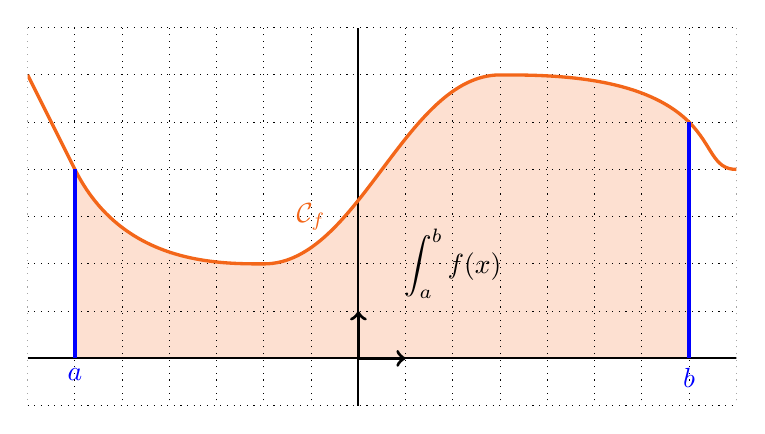
\begin{tikzpicture}[scale=0.6]
\clip (-7,-1) rectangle (8,7);

\filldraw [draw=black,fill=ocre!20]
(-6,4) .. controls (-5,2) and (-3,2) .. (-2,2)
.. controls (0,2) and (1,6) .. (3,6) .. controls (4,6) and (6,6) ..
(7,5) -- (7,0) -- (-6,0) -- cycle;

\draw [ thin, dotted] (-7,-3) grid (9,7);
\draw [thick] (-7,0)--(9,0);
\draw [thick] (0,-3)--(0,7);
\draw [->, very thick] (0,0)--(1,0);
\draw [->,very thick] (0,0)--(0,1);

\draw [ocre, very thick] (-7,6) .. controls (-6.5,5) and (-7,6).. (-6,4) .. controls (-5,2) and (-3,2) .. (-2,2)
.. controls (0,2) and (1,6) .. (3,6) .. controls (4,6) and (6,6) ..
(7,5) ..controls (7.5,4.5) and (7.5,4) .. (8,4);

\draw [blue, very thick] (7,0) -- (7,5);
\draw [blue, very thick] (-6,0) -- (-6,4);

\draw [ocre] (-1,3) node {$\mathcal{C}_f$};
\draw [blue] (-6,0) node[below] {$a$};
\draw [blue] (7,0) node[below] {$b$};
\draw (2,2) node {$\displaystyle\int_a^b f(x)\dx$};


\end{tikzpicture}
\end{center}

\begin{example}Il est possible d'encadrer l'aire sous la courbe en utilisant le quadrillage. 

Ici, l'aire sous la courbe est composée de 44 carreaux entiers, l'intégrale est donc supérieur ou égale à 44. Par ailleurs, si on ajoute les 17 carreaux que traverse la courbe, on a alors que l'intégrale est inférieure à 61. 

On a alors  $44 \leqslant \displaystyle\int_{a}^b f(x)\dx \leqslant 61$.\end{example}

La notation de l'intégrale est due à Leibniz : pour calculer l'aire sous une courbe, Leibniz l'approchait par des rectangles de largeur de plus en plus petite. La hauteur des rectangles en $x$ était $f(x)$ et leur largeur, notée $\dx$, se rapprochait de 0 : on faisait donc la somme des $f(x)\dx$ entre $a$ et $b$. Le symbole $\int$ de l'intégrale n'est autre qu'un $S$ allongé qui signifie justement "somme".


\begin{center}

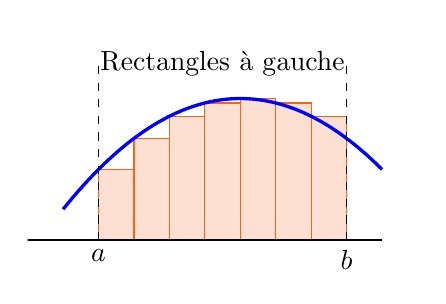
\begin{tikzpicture}[scale=0.45]
\clip (-1,-1) rectangle (10,6);
\draw (4.5,5) node {Rectangles à gauche};
\foreach \k in {1,2,...,7} {\draw [ocre,fill=ocre!20] (\k,0)--(\k,-0.125*\k*\k+1.25*\k+0.875) -- (\k+1,-0.125*\k*\k+1.25*\k+0.875) -- (\k+1,0) -- cycle;}

\draw [thick] (-6,0)--(9,0);
\draw [blue, very thick,domain=0:9,samples=100] plot (\x,{-0.125*\x*\x+1.25*\x+0.875});

\draw [dashed] (1,0)--(1,5);
\draw [dashed] (8,0)--(8,5);
\draw (8,0) node[below] {$b$};
\draw (1,0) node[below] {$a$};
\end{tikzpicture}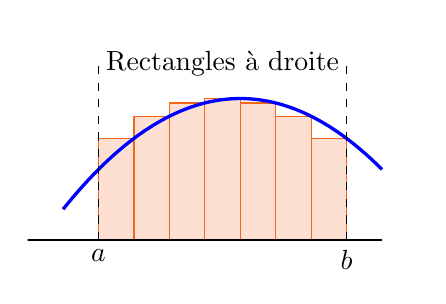
\begin{tikzpicture}[scale=0.45]
\clip (-1,-1) rectangle (10,6);
\draw (4.5,5) node {Rectangles à droite};
\foreach \k in {2,3,...,8} {\draw [ocre,fill=ocre!20] (\k,0)--(\k,-0.125*\k*\k+1.25*\k+0.875) -- (\k-1,-0.125*\k*\k+1.25*\k+0.875) -- (\k-1,0) -- cycle;}

\draw [thick] (-6,0)--(9,0);
\draw [blue, very thick,domain=0:9,samples=100] plot (\x,{-0.125*\x*\x+1.25*\x+0.875});

\draw [dashed] (1,0)--(1,5);
\draw [dashed] (8,0)--(8,5);
\draw (8,0) node[below] {$b$};
\draw (1,0) node[below] {$a$};
\end{tikzpicture}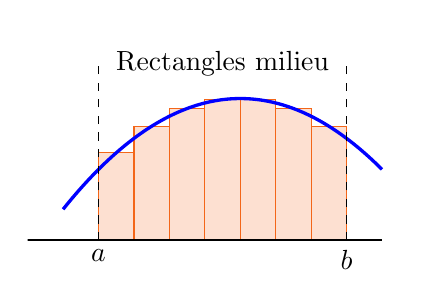
\begin{tikzpicture}[scale=0.45]
\clip (-1,-1) rectangle (10,6);
\draw (4.5,5) node {Rectangles milieu};
\foreach \k in {1.5,2.5,...,7.5} {\draw [ocre,fill=ocre!20] (\k-0.5,0)--(\k-0.5,-0.125*\k*\k+1.25*\k+0.875) -- (\k+0.5,-0.125*\k*\k+1.25*\k+0.875) -- (\k+0.5,0) -- cycle;}

\draw [thick] (-6,0)--(9,0);
\draw [blue, very thick,domain=0:9,samples=100] plot (\x,{-0.125*\x*\x+1.25*\x+0.875});

\draw [dashed] (1,0)--(1,5);
\draw [dashed] (8,0)--(8,5);
\draw (8,0) node[below] {$b$};
\draw (1,0) node[below] {$a$};
\end{tikzpicture}

\end{center}

\begin{example} Pour tout réel $x$, on pose $f(x)=6-2x$. On cherche la valeur de $\displaystyle\int_{-2}^1 f(x)\dx$.


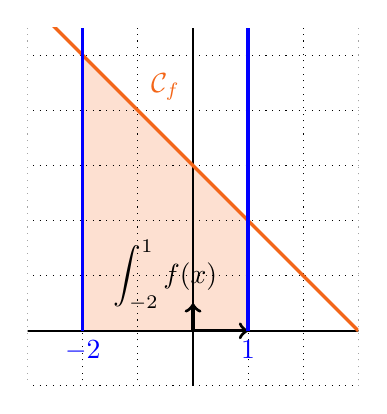
\begin{tikzpicture}[scale=0.7,x=1cm, y=0.5cm]
\clip (-3,-2) rectangle (3,11);

\filldraw [draw=black,fill=ocre!20]
(-2,0) --(1,0) -- (1,4) -- (-2,10) -- cycle;

\draw [ thin, dotted] (-7,-3) grid (9,11);
\draw [thick] (-7,0)--(9,0);
\draw [thick] (0,-3)--(0,11);
\draw [->, very thick] (0,0)--(1,0);
\draw [->,very thick] (0,0)--(0,1);

\draw [ocre, very thick, domain=-3:3] plot (\x,{6-2*\x});

\draw [blue, very thick] (-2,0) -- (-2,11);
\draw [blue, very thick] (1,0) -- (1,11);

\draw [ocre] (-0.5,8) node[above] {$\mathcal{C}_f$};
\draw [blue] (-2,0) node[below] {$-2$};
\draw [blue] (1,0) node[below] {$1$};
\draw (-0.5,2) node {$\displaystyle\int_{-2}^1 f(x)\dx$};


\end{tikzpicture}



\end{example}

\begin{proposition}Si $f$ et $g$ sont deux fonctions continues sur $[a,b]$.

On suppose que pour tout réel $x\in[a,b]$, on a $f(x) \geqslant g(x)$.

L'aire délimitée par les courbes de $f$ et de $g$ ainsi les droites d'équation $x=a$ et $x=b$ vaut $\displaystyle\int_{a}^b (f-g)(x)\dx$.\end{proposition}

Il est alors possible de déterminer l'aire entre deux courbes sans même savoir l'aire sous chacune de ces deux courbes.

\begin{example}Pour tout réel $x$, on pose $f(x)=\dfrac{x^2}{4}+\dfrac{x}{3}+1$ et $g(x)=\dfrac{x^2}{4}-\dfrac{x}{2}+1$.\\ On souhaite déterminer l'aire entre les courbes de $f$ et $g$ entre les abscisses 0 et 3.


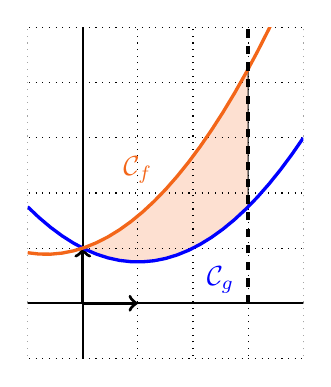
\begin{tikzpicture}[scale=0.7]
\clip (-1,-1) rectangle (4,5);

\filldraw [draw=black,fill=ocre!20]
plot [domain = 0:3] (\x,{\x*\x/4-\x/2+1}) -- (3,17/4) -- plot [domain = 3:0] (\x,{\x*\x/4+\x/3+1}) -- cycle;


\draw [ thin, dotted] (-7,-3) grid (9,11);
\draw [thick] (-7,0)--(9,0);
\draw [thick] (0,-3)--(0,11);
\draw [->, very thick] (0,0)--(1,0);
\draw [->,very thick] (0,0)--(0,1);

\draw [blue, very thick, domain=-1:4] plot (\x,{\x*\x/4-\x/2+1});
\draw [ocre, very thick, domain=-1:4] plot (\x,{\x*\x/4+\x/3+1});


\draw [dashed, very thick] (3,0) -- (3,6);

\draw [ocre] (1,2) node[above] {$\mathcal{C}_f$};
\draw [blue] (2.5,0) node[above] {$\mathcal{C}_g$};

\end{tikzpicture}

\vskip150pt

\end{example}
\newpage
\section{Intégrale et primitives}
\subsection{Théorème fondamental}

\begin{theorem}
 $f$ une fonction continue et positive sur $[a,b]$. 
 
La fonction $F_a:x\mapsto \displaystyle\int_{a}^x f(t)dt$ est la primitive de $f$ qui s'annule en $a$.

En particulier, toute fonction continue positive admet une primitive.\end{theorem}

\begin{demonstration} On se contente de démontrer le cas où $f$ est strictement croissante sur l'intervalle $[a;b]$.

\end{demonstration}
\newpage

\begin{definition}Soit $f$ une fonction continue et positive sur $[a,b]$ et $F$ une primitive de $f$ sur cet intervalle.
 \[\displaystyle\int_{a}^b f(x)\dx=F(b)-F(a).\]
 On note également $[F(x)]_a^b$.\end{definition}
 
\begin{demonstration} On considère la fonction $F_a:x\mapsto \displaystyle\int_{a}^x f(t)dt$. On rappelle que cette fonction est l'unique primitive de $f$ sur $[a;b]$ qui s'annule en $a$. 

\vskip150pt

\end{demonstration}
 
Cette quantité ne dépend donc pas de la primitive choisie !
 
\begin{example}On cherche à calculer  $\displaystyle\int_{1}^5 x^2 \dx $.

\vskip40pt
\end{example}
 

\subsection{Généralisation aux fonctions de signe quelconque}

\begin{definition}Soit $f$ une fonction continue sur $[a,b]$ et $F$ une primitive de $f$ sur cet intervalle. On définit l'intégrale de $f$ sur $[a,b]$ par \[\displaystyle\int_{a}^b f(t)dt = F(b)-F(a).\]\end{definition}

\begin{example} On cherche à calculer $\displaystyle\int_{-2}^1 x^3 \dx$.
\vskip40pt
\end{example}

 \newpage

La quantité ici est négative, il n'est pas possible de l'interpréter directement comme une aire. Il s'agit en réalité de la différence de l'aire entre la courbe et l'axe des abscisses lorsque la courbe est au-dessus de cet axe et de cette même aire lorsque la courbe est cette fois en-dessous de l'axe des abscisses.
\begin{center}
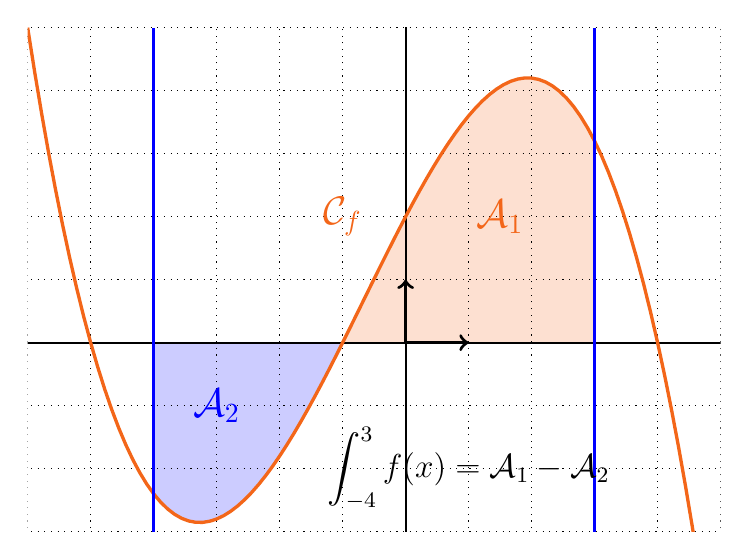
\begin{tikzpicture}[scale=0.8]
\clip (-6,-3) rectangle (5,5);

\filldraw [draw=black,fill=ocre!20]
plot [domain = -1:3] (\x,{-(\x+5)*(\x+1)*(\x-4)/10}) -- (3,0) -- cycle;

\filldraw [draw=black,fill=blue!20]
plot [domain = -1:-4] (\x,{-(\x+5)*(\x+1)*(\x-4)/10}) -- (-4,0) -- cycle;


\draw [ thin, dotted] (-7,-4) grid (9,7);
\draw [thick] (-7,0)--(9,0);
\draw [thick] (0,-4)--(0,7);
\draw [->, very thick] (0,0)--(1,0);
\draw [->,very thick] (0,0)--(0,1);

\draw [ocre, very thick, domain=-6:5, samples=100] plot (\x,{-(\x+5)*(\x+1)*(\x-4)/10});

\draw [blue, very thick] (-4,-4) -- (-4,5);
\draw [blue, very thick] (3,-4) -- (3,5);

\draw [ocre] (-1,2) node {{\Large $\mathcal{C}_f$}};
\draw [ocre] (1.5,2) node {{\Large $\mathcal{A}_1$}};
\draw [blue] (-3,-1) node {{\Large $\mathcal{A}_2$}};

\draw (1,-2) node {{\large $\displaystyle\int_{-4}^3f(x)\dx=\mathcal{A}_1-\mathcal{A}_2$}};


\end{tikzpicture}
\end{center}



\subsection{Propriétés de l'intégrale}

 \begin{proposition}Soit $f$ et $g$ deux fonctions continues sur un intervalle $[a,b]$ et $c$ un réel de l'intervalle $[a,b]$. Soit $\lambda$ réel.
 
 \begin{itemize}
 \item $\displaystyle\int_{a}^b (f+g)(t)dt=\displaystyle\int_{a}^b f(t)dt+\displaystyle\int_{a}^b g(t)dt$ ;
 \item $\displaystyle\int_{a}^b \lambda f(t)dt=\lambda\displaystyle\int_{a}^b f(t)dt$ ;
 \item \textbf{(Relation de Chasles)} $\displaystyle\int_{a}^c f(t)dt+\displaystyle\int_{c}^b f(t)dt = \displaystyle\int_{a}^b f(t)dt$.
 \end{itemize}\end{proposition}
 
 La relation de Chasles permet notamment de calculer la valeur d'intégrales de fonctions définies par morceaux.
 
\begin{example} On considère la fonction $f$ définie pour tout réel $x$ par \renewcommand{\arraystretch}{1}$f(x)=\left\{\begin{array}{ll} x^2+1&,\text{ si }x<0\\ x^3+1&,\text{ si }x\geqslant 0\end{array}\right.$.

La fonction $f$ est continue sur $[-2;3]$. En effet, le seul souci en éventuel se situe en 0. 

Or, $\displaystyle\lim_{x\to 0^-} f(x)= 0^2+1=1$, $\displaystyle\lim_{x\to 0^+} f(x)= 0^3+1=1$ et $f(0)=1$. Ainsi,
 \[\displaystyle\int_{-2}^3 f(x)\dx=\]
 
 Or, une primitive de $x\mapsto x^2+1$ sur $[-2,0]$ est $x\mapsto \dfrac{x^3}{3}+x$ et une primitive de $x\mapsto x^3+1$ sur $[0;3]$ est $x\mapsto \dfrac{x^4}{4}+x$. Finalement,
 
 \[\displaystyle\int_{-2}^3 f(t)dt=\left[\dfrac{x^3}{3}+x\right]_{-2}^0+\left[\dfrac{x^4}{4}+x\right]_0^3=\dfrac{14}{3}+\dfrac{93}{4}=\dfrac{335}{12}.\]\vspace{-0.5cm}\end{example}



\begin{proposition} Soit $f$ une fonction continue sur $[a,b]$.

Si pour tout réel $x$ dans $[a,b]$, $f(x)\geqslant 0$, alors $\displaystyle\int_{a}^b f(x)\dx \geqslant 0$.
\end{proposition}

Cette propriété est souvent utilisée dans le sens contraposé : si $f$ est une fonction continue et positive d'intégrale nulle, alors $f$ est la fonction nulle.

\begin{proposition} Soit $f$ et $g$ deux fonctions continues sur $[a,b]$ telles que pour tout réel $x$, $f(x)\leqslant g(x)$.

On a alors $\displaystyle\int_{a}^b f(x)\dx\leqslant \displaystyle\int_{a}^b g(x)\dx$.\end{proposition}

\begin{demonstration} La fonction $g-f$ est continue et positive sur $[a,b]$. 

Ainsi, d'après la propriété précédente, $\displaystyle\int_{a}^b(g- f)(x)\dx \geqslant 0$. 

Or, $\displaystyle\int_{a}^b (g-f)(x)\dx=\displaystyle\int_{a}^b g(x)\dx-\displaystyle\int_{a}^b f(x)\dx \geqslant 0$. On a donc $\displaystyle\int_{a}^b f(x)\dx \leqslant \displaystyle\int_{a}^b g(x)\dx$.\end{demonstration}

\begin{example}Soit $f$ une fonction continue sur $[-2,5]$ telle que pour tout $x\in [-2;5]$, on a $x\leqslant f(x) \leqslant 7$.


\vskip100pt

\end{example}

\subsection{Valeur moyenne d'une fonction}

\begin{definition} Soit $f$ une fonction continue sur un intervalle $[a,b]$.

On appelle valeur moyenne de $f$ sur $[a,b]$ le réel \[m=\dfrac{1}{b-a}\displaystyle\int_{a}^b f(x)\dx.\]\end{definition}

\begin{example}La valeur moyenne de la fonction $f:x\mapsto x^2+1$ sur [1;4] vaut
\[ \dfrac{1}{4-1} \int_{1}^4 (x^2+1)\dx = \dfrac{1}{3}\left[ \dfrac{x^3}{3}+x\right]^4_1=\dfrac{1}{3}\left(\dfrac{4^3}{3}+4-\dfrac{1^3}{3}-1\right)=24.\]\vspace{-0.5cm}\end{example}


\begin{minipage}{0.65\linewidth}
Pourquoi le nom de valeur moyenne ? Si l'on note $M$ la valeur moyenne de la fonction $f$, alors l'aire sous la courbe de $f$ entre $a$ et $b$ correspond à l'aire du rectangle ayant pour longueur $b-a$ et pour hauteur $M$.

Dans le cas ci-contre, le rectangle hachuré (qui a pour hauteur la valeur moyenne de la fonction représentée) et le domaine rempli en rouge ont la même aire.\end{minipage}\hfill\begin{minipage}{0.3\linewidth}

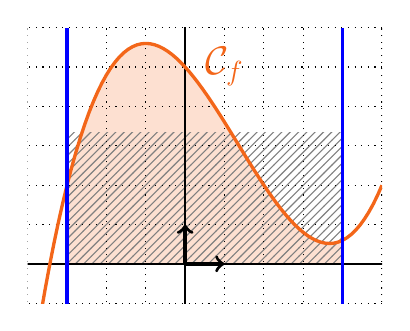
\begin{tikzpicture}[scale=0.5]
\clip (-4,-1) rectangle (5,6);



\filldraw [draw=black,fill=ocre!20]
plot [domain = -3:4] (\x,{(\x+3)*(\x-2)*(\x-5)/10+2}) -- (4,0) -- (-3,0) -- cycle;

\fill [pattern=north east lines, pattern color = gray, distance = 3]
(-3,0) -- (-3,3.34) -- (4,3.34) -- (4,0)-- cycle;


\draw [ thin, dotted] (-7,-4) grid (9,7);
\draw [thick] (-7,0)--(9,0);
\draw [thick] (0,-4)--(0,7);
\draw [->, very thick] (0,0)--(1,0);
\draw [->,very thick] (0,0)--(0,1);

\draw [ocre, very thick, domain=-6:5, samples=100] plot (\x,{(\x+3)*(\x-2)*(\x-5)/10+2});

\draw [blue, very thick] (-3,-4) -- (-3,6);
\draw [blue, very thick] (4,-4) -- (4,6);

\draw [ocre] (1,5) node {{\Large $\mathcal{C}_f$}};



\end{tikzpicture}

\end{minipage}



\section{Intégration par parties}

\begin{proposition}Soit $u$ et $v$ deux fonctions dérivables sur un intervalle $[a,b]$ dont la dérivée est continue sur cet intervalle. Alors
\[\displaystyle\int_{a}^b (uv')(x)\dx=[uv]_a^b-\displaystyle\int_{a}^b (u'v)(x)\dx.\]\end{proposition}

\begin{demonstration}$uv$ est dérivable sur $[a,b]$ comme produit de fonctions dérivables sur cet intervalle. D'après la formule de dérivée d'un produit, $(uv)'=u'v+uv'$, c'est-à-dire $uv'=(uv)'-u'v$. En intégrant cette égalité entre $a$ et $b$, on obtient le résultat voulu.\end{demonstration}

\begin{example} On souhaite calculer $\displaystyle\int_{0}^1x\e^{2x} \dx$.

\vskip200pt

\end{example}

L'intégration par parties est pour la première fois abordée par Brook Taylor en 1715, dans son livre \textit{Methodus Incrementorum directa et inversa}. Dans cet ouvrage, Taylor utilise la notation de Newton : les dérivées sont symbolisées par un point et les intégrales par un rectangle qui entoure la fonction. 

\begin{center}
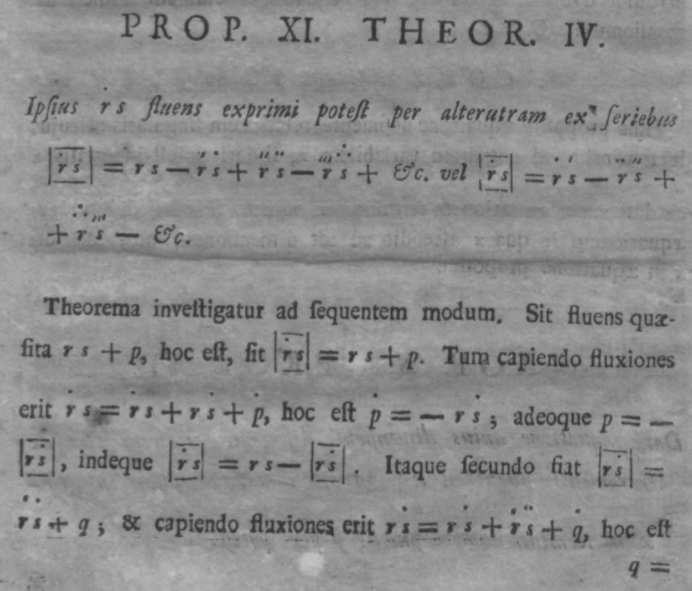
\includegraphics[scale=0.4]{taylor}
\end{center}






\end{document}